\begin{frame}
	\frametitle{Alberi di Merkle}
	
\begin{columns}
 \begin{column}{.72\textwidth}

		usati in protezione {\color{blue}integrità transazioni} %�
		\begin{itemize}
			\item foglia $\leftrightarrow\; \mathfrak{T}$
			\item $\neg$ foglia $\leftrightarrow$ hash dei due figli
			\vspace{5pt}
			\item decidere se una foglia $\in$ 
			\begin{itemize}
				\item lista: $O(\orange{N})$
				\item albero: $O(\orange{\log_2 N}) \ll O(N)$
				
			\end{itemize}
			\vspace{5pt}
			\item Bitcoin: $\;\mathrm{hash}(\orange{n})=SHA_{256}(SHA_{256}(\orange{\mathcal{L}_n}|\orange{\mathcal{R}_n}))$
		\end{itemize}

	\end{column}

	\begin{column}{.4\textwidth}
		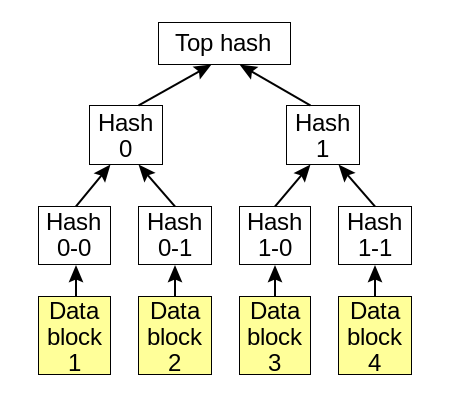
\includegraphics[height = 4 cm]{images/merkle.png}
	\end{column}
\end{columns}

\end{frame}